%
% The Current Maintainer of this work is Paul Vojta.

\documentclass[phd]{ucbthesis}
\usepackage{biblatex}
\usepackage{color}
\usepackage{graphicx}
\usepackage{subcaption}
\usepackage{siunitx}
\usepackage{listings}
\usepackage{rotating}
\usepackage{multirow}
\usepackage{xspace}

% To compile this file, run "latex thesis", then "biber thesis"
% (or "bibtex thesis", if the output from latex asks for that instead),
% and then "latex thesis" (without the quotes in each case).

% Double spacing, if you want it.  Do not use for the final copy.
\def\dsp{\def\baselinestretch{1.5}\large\normalsize}
%\dsp

% If the Grad. Division insists that the first paragraph of a section
% be indented (like the others), then include this line:
% \usepackage{indentfirst}

% commands
\newcommand{\ignore}[1]{}
\newcommand{\TODO}[1]{{\color{red}\textbf{TODO: #1}}}
\newcommand{\RISCV}{\mbox{RISC-V}}
\newcommand{\wunits}[2]{\mbox{#1\,#2}}

% commands use to alias tbd names
% Paper name
\newcommand{\PNAME}{\mbox{\textsc{fased}}\xspace}
% Simulation framework name
\newcommand{\SIMNAME}{MIDAS\xspace}

\bibliography{refs}

% Increase the depth of numbering sections

\hyphenation{Rocket-Chip MIDAS}
\begin{document}

% Declarations for Front Matter

\title{FPGA-Accelerated Simulation of ASICs with Dynamically Scaling Clocks}
\author{David Thomas Biancolin}
\degreesemester{Spring}
\degreeyear{2019}
\degree{Doctor of Philosophy}
\chair{Professor Krste Asanovi\'c}
\cochair{Adjunct Professor Jonathan Richard Bachrach}
\othermembers{Professor Sanjit Seshia \\ Professor Robert Leachman }
% Previous degrees are no longer to be listed on the title page.
% \prevdegrees{B.A. (University of Northern South Dakota at Hoople) 1978 \\
%   M.S. (Ed's School of Quantum Mechanics and Muffler Repair) 1989}
\field{Electrical Engineering and Computer Science}
% Designated Emphasis -- this is optional, and rare
% \emphasis{Colloidal Telemetry}
% This is optional, and rare
% \jointinstitution{University of Western Maryland}
% This is optional
\campus{Berkeley}

% For a masters thesis, replace the above \documentclass line with
% \documentclass[masters]{ucbthesis}
% This affects the title and approval pages, which by default calls this
% document a "dissertation", not a "thesis".

% A slightly modified template of the ms thesis to reuse the title variables
\clearpage
%\input{tex/cover}
\maketitle
% Delete (or comment out) the \approvalpage line for the final version.
%\approvalpage
\copyrightpage
% (Optional) \part{First Part}

\begin{abstract}
%While specialization appears to be only path towards higher performance and more
energy efficient computer hardware, the enormous non-recurring engineering (NRE) cost
of designing modern systems-on-a-chip~(SoCs) is a major barrier to the wider
adoption of custom silicon. As part of a larger effort exploring more
cost-effective agile methodologies for designing custom silicon, this work
contributes to a novel \emph{single-FPGA} hardware emulation framework, FireSim, that aims to
radically reduce the cost of doing fast and accurate full-system simulation.

In this dissertation, we start by introducing a compiler infrastructure, called
\texttt{Golden Gate}, capable of performing general multi-cycle resource
optimizations in order to fit larger SoCs on a single FPGA. The
nature of these optimizations is described at length in A. Magyar's
dissertation~\cite{MagyarDissertation}. Using this compiler infrastructure, we
study optimization-compatible schemes for simulating SoCs with more realistic
clocking organizations.  We first present a simple approach for simulating
systems with multiple fixed-frequency clocks.  We then extend this to support a
more general class of clock switching and generation behavior, notably to
enable timing-exact simulation dynamic frequency scaling. Our approach is based
on prior work in software-based, conservative parallel-discrete event
simulation wherein we replace clock switching and generation structures, like
clock multiplexors, with decoupled models that act on timestamped message
streams.  Unlike other academic FPGA-based systems, which tend to be FPGA
prototypes that rely on direct instantiation of FPGA clocking primitives, here
we strictly use clock gating to derive simulated clocks, making our approach
far easier to use and FPGA portable.

\end{abstract}

\begin{frontmatter}
% You can delete the \clearpage lines if you don't want these to start on
% separate pages.

\setcounter{tocdepth}{2}
\setcounter{secnumdepth}{2}
\tableofcontents
\clearpage
\listoffigures
\clearpage
\listoftables
\begin{acknowledgements}
\end{acknowledgements}
\end{frontmatter}

\pagestyle{headings}


%\chapter{Introduction}
%
%%Today, the semiconductor industry finds itself in the midst of a storm emerging
from two colliding fronts\footnote{I borrow this metaphor from my advisor,
Krste Asanovi\'c.}. The first
of these, the hot front, is an exponential growth in the diversity and volume
of computing applications.  While AI, specifically machine
learning, has captured the zeitgiest, advances in semiconductor process
technologies have made it possible to embed computing in nearly all aspects of
human life. This manifests at the extremes as deeply embedded systems, often running in highly
energy-constrained environments, and cloud-hosted services, running in
multi-megawatt-scale datacenters, all interconnected via an evermore capable internet.  All of
this---from the smallest embedded microcontrollers to the largest
datacentered-oriented servers, and the networking hardware that connects
them---runs on transistor technologies whose fundamental physics have not
changed since the mid-twentieth century.

Indeed, the ``cold" front of this storm is the inevitable slowing of transistor
scaling trends that have long been the hallmark of the semiconductor industry.
First, we lost Dennard scaling~\cite{DennardScaling}: a regime in which a
shrink in transistor channel length and voltage would produce a proportional
reduction in the delay of a circuit built from them.  Dennard scaling drove an
era of exponential increase in computing performance wherein one could simply
reimplement an existing design in the latest process technology to realize
large speedups. Dennard scaling ended in the mid-aughts when it became
difficult to further  scale transitor voltages without losing the ability to
shut them off~\cite{ScalingChallenges}, forcing power density to increase. This
put a thermal limit on how fast one could clock a chip and led microprocessor
manufacturers to abandon development of higher-frequency, deeply pipelined
machines.

In the years since, advances in computing performance have ridden on the back
of the industry's better-known scaling trend, Moore's Law~\cite{MooresLaw}. Even if
transistors were not getting faster, they were still shrinking. These extra
transistors could be translated into larger caches and prediction structures,
physically wider vector and SIMD intruction pipelines, and most notably, more
processor cores. In this time, we also saw the rise of the general-purpose
GPU~(GPGPU), whose more parallel architecture scales naturally to use more
transistors than a conventional microprocessor. GPGPUs have been
a fundamental driver in the success of many modern machine-learning
techniques~\cite{AlexNet}.  Unfortunately, GPGPUs are far from truly
general-purpose; the bulk of the world's applications still run on conventional
microprocessors where improvements offered by more cores and other
microarchitectural enchanchments are bearing less fruit.

With no radically better general-purpose computer architecture (based in
silicon or otherwise) waiting in the wings, there is broad agreement that only means to deliver continued advances in
computing performance and energy efficiency is with specialization. In
academia, many researchers are building accelerators
for specific application domains, like graph computing~\cite{Graphicionado}
and machine learning~\cite{Eyeriss}. In industry, there is a growing number of
companies designing there own silicon where previously they would have
purchased offerings from existing players. Notable
examples include Tesla~\cite{FSDChip}, Amazon~\cite{Graviton},
Google~\cite{TPU}, and mostly recently, Apple\footnote{Apple has long been
designing its own SoCs for its mobile phones, but used Intel SoCs in their laptops and desktops.} with their M1
SoC~\cite{AppleM1}.

What this ``specialization" should look like is the defining question
of this era of computer architecture research. However, the more narrow concern of
this dissertation is how a particular microarchitecture should be implemented in silicon.  While
application-specific integrated circuits (ASICs), offer the best potential for
realizing these improvements, the non-recurring engineering~(NRE) cost of a new
design is enormous and growing~(Figure~\ref{fig:chip-nre}). As a result, reconfigurable logic devices like
field-programmable gate arrays~(FPGAs) have long filled low-volume niches where
the NRE of custom silicon~(i.e., an ASIC) cannot be effectively amortized. The need for
lower cost, energy-efficient hardware has also driven a resurgance in
structured ASICs~\cite{SAHARA}: these are FPGA-like devices whose
field-programability has been removed. Structured ASICS attempt to close the performance and
energy-efficiency gap between FPGAs and ASICs while saving up to 90 \% of the
NRE of an equivalent ASIC~\cite{StructuredASIC}.  Nonetheless, we believe the
performance and energy-efficiency costs~\cite{FPGAGap2} of using these
intermediate technologies is large enough to justify a redoubled effort to make
standard-cell-based ASIC design more economical.

The large NRE of developing an ASIC is in part historical.  Years of
advantagenous scaling trends have bred a business model into the industry in
which, at least in advanced technologies, relatively few unique designs are
taped out in enormous volumes. Simultaenously, advances in general-purpose computers dissuaded
investment in smaller-volume custom-silicon projects: why, after all, would one
design an ASIC, when one could wait two years for the next Intel CPU?
As a result, tools and metholodogies have been designed and optimized around
large NREs and large volumes to amortize them. Moreover, the established
players in the electronic design automation~(EDA) industry, responsible for
developing the tools used to design ASICs, are exceptionally profitable and have little short-term
incencitive to alter this business model. For the benefits of custom silicon to be attainable for
the non-Apples and Googles of the world this will need to change.

\begin{figure}
    \centering
    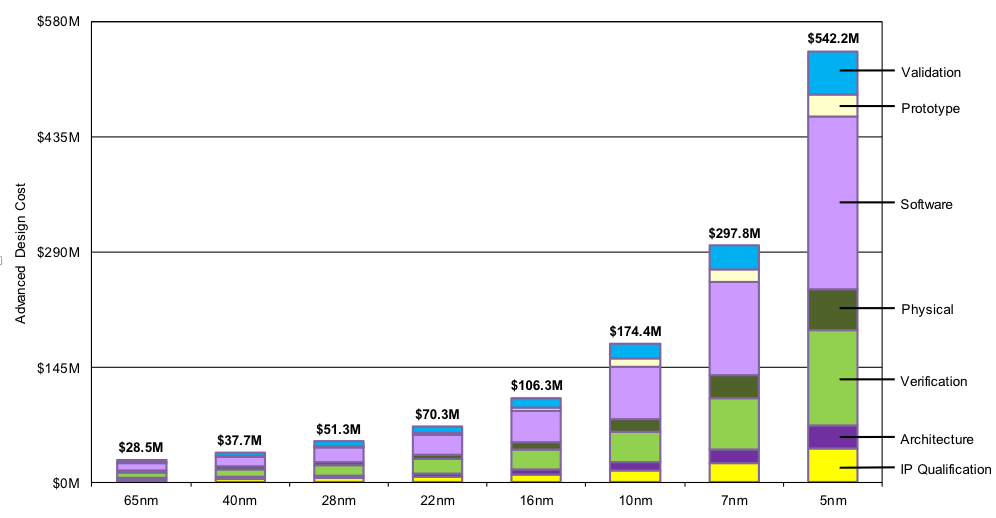
\includegraphics[width=0.99\textwidth]{figures/nre-cost.png}
    \caption{Early design non-recurring engineering~(NRE) cost
    at various feature dimensions. Source: IBS.}
    \label{fig:chip-nre}
\end{figure}

Part of the problem is that there appears to be no silver bullet for reducing
ASIC NRE, as there many disparate sources that often span multiple domains of
chip design~(Figure~\ref{fig:chip-nre}). Instead, we will need many diverse
tooling improvements united under a reimagined methodology for building custom
silicon. At Berkeley, we have articulated one such vision inspired by agile
software-engineering practises~\cite{AgileHW} and have built tools to support it.
These tools include Chisel~\cite{Chisel}, a more productive hardware-design
language (HDL) based in Scala, and FIRRTL~\cite{FIRRTL}, a flexible
intermediate representation for hardware that makes it easier to build
compilers. Perhaps the largest contribution to this vision has been the RISC-V
instruction set architecture~(ISA)~\cite{WatermanDissertation}.  Being open and
free-to-use, RISC-V enables chip designers to build customized microprocessors
while extending an open-source software toolchain.  This avoids the costs and
legal encumbarances of using a priopreitary ISA, or the massive engineering
burden of developing a fully custom ISA. RISC-V adoption has been meteoric in
recent years, both in academia outside of Berkeley~\cite{BlackParrot, Celerity,
Pulp}, and in industry, where a growing body of companies, notably SiFive,
Western Digital, and Nvidia have been developing new RISC-V implementations.

One unaddressed deficiency in chip design that drives verification, validation and software development
costs, is the lack of a good full-system simulation technology. Ideally, such
a technology would be:
\begin{itemize}
    \item \textbf{Fast.} As fast as silicon prototype, so as to enable running full system
    stacks and complete applications.
\item \textbf{Detailed.} It would simulate SoC's timing characteristics exactly.
\item \textbf{Productive.} It would be easy to debug and fast to recompile.  It would feel much like a software-based simulator.
\item \textbf{Inexpensive.} It would be cheap to deploy so that it could be made widely accessible
        to hardware and software design teams and support running large parallel experiments.
\end{itemize}

In practise, existing simulation technologies are forced to prioritize two of
these objectives. Software simulators, despite being easy to use and relatively
inexpensive, are much too slow to run full-system simulations when providing a
cycle-accurate model of the chip. For speed, chip designers are forced to turn
to hardware acceleration, in the form of FPGA prototyping and hardware
emulation.  Of the two, FPGA prototypes tend to be faster and less expensive,
and so see extensive use in software development and regression testing later
in the design cycle.  Conversely, hardware emulation is slower and considerably
more expensive, but offers a software-simulator-like debugging experience that
makes it a critical tool for pre-silicon verification. We will expand more on these
differences in Chapter~\ref{sec:simulation-background}.

The central question of the simulation work underway at Berkeley asks if it is
possible to build a simulation platform that can marry the speed of FPGA
prototyping, and the productivity of hardware emulation, while being radically
cheaper to deploy. Such a technology would put hardware emulation in the hands
of smaller research groups, and make it more widely available in companies
where scarse emulation resources must be carefully scheduled. Additionally, if
it is fast enough, it could subsume the role of a conventional FPGA prototype,
reducing the engineering burden of having parallel emulation and FPGA
prototyping infrastructures. If this technology is going to be inexpensive, two
things are clear.  First, it must use commericial off-the-shelf~(COTS) FPGA
platforms, and not custom devices or system integration as is true of all
commerical emulators. Second, this technology's software ecosystem, including
tools and IP libraries, will need to be open-source with the hope that they can
be developed and maintained by a community of users instead of a private team
of engineers.

This is no small undertaking but one made easier by recent technology trends.
Firstly, modern FPGAs are enormous, continue to be amoung the greatest
beneficiaries of Moore's law since they can naturally scale to use larger
transistor budgets. Advances in multi-die integration technologies have made
it easier to reliably manufacture even larger FPGAs. This makes it possible to
simulate considerably larger systems on a single FPGA.  Secondly, FPGAs are now available
in public cloud and provided by many major vendors like Amazon Web Services~\cite{amazonf1}.
This means a team can avoid the expense of building and
maintaining their own local FPGA cluster, and can use newer FPGAs as they
become available. Cloud services also provide an elastic supply of FPGAs,
allowing users to scale out experiments as needed, instead of needing to
provision a local cluster for the worst case. While the rates of using
cloud-based FPGAs are currently non-trivial, we expect these to fall in the
future as the costs of these services are amortized. Finally, it would be
difficult to build out an emulation infrastucture without the aforementioned advances in
open-source tooling. A compiler lies at the heart of all hardware emulation systems:
FIRRTL and its and Scala-based compiler infrastructure provide flexible
abstractions for translating a design into an FPGA-hosted emulator. FPGA-hosted emulation
infrastucture requires customized hardware, and more productive hardware-design
languages, like Chisel, makes it considerably easier for a small team to build
it. Finally, for an open-source infrastructure to see use, it
requires open-source input designs to both encourage adoption and inform
development. Here, we can leverage a growing body of RISC-V based processors,
such as Rocket~\cite{RocketChip} and BOOM~\cite{BOOM}, to feed into our system.

While it initially began as a project to study warehouse-scale computers, the
FireSim~\cite{FireSim} project has been our attempt at building out this
new technology. FireSim has been the basis for a
number of emulation-related research papers at Berkeley: we have studied
detailed DRAM timing models~\cite{FASED}, non-invasive, full-system profiling
techniques~\cite{FirePerf}.  FireSim-adjacent projects, using the same
underlying compiler, MIDAS~\cite{MIDAS}, have explored novel techniques for rapid
debugging~\cite{DESSERT}, and energy estimation~\cite{Simmani, Strober}. Over
time, features from these projects have gradually been integrated in mainline
FireSim, where they are employed by a growing user base.

Unfortunately, limitations with MIDAS limited its scope
to simple designs. First, these designs were small: they could be directly
implemented on a single Xilinx Ultrascale+ VU9P FPGA. In contrast, FPGA prototypes
of modern SoCs require partitioning over multiple FPGAs~\cite{FPMM}.  Second, these systems possessed only a single
clock domain. Conversly, modern SoCs have dozens of clocks whose frequencies
may change during execution. Without the ability to simulate
even a small number of fixed-frequency clocks it was difficult to get truly
accurate performance estimates with FireSim. Addressing these two challenges
drove the design of a new optimizing-compiler called Golden Gate~\cite{GoldenGate}.

To simulate larger systems, Golden Gate uses multi-cycle resource optimizations
to replace FPGA-hostile blocks. Golden Gate automates many techniques
deployed in prior academic work in FPGA-accelerated microarchitecture
simulation to radically improve the capacity of single FPGA. These
optimizations are the focus of Albert Magyar's dissertation~\cite{MagyarDissertation}.
Addressing the second challenge of simulating systems with more realistic clock
organizations is the subject of this dissertation. The contribution of this
work are threefold:

\begin{enumerate}
\item We describe Golden Gate, an optimizing compiler infratructure to deploy module-based
    multi-cycle resource optimizations~(Chapter~\ref{sec:golden-gate}. This
    contribution is shared with Albert Magyar, and is also described in his
    dissertation.

\item A simple, FPGA-flexible, extension to Golden Gate to support systems
    with fixed frequency clocks that is compatible with multi-cycle resource optimizations~(Chapter~\ref{sec:static-multiclock}).

\item A general, distributed approach for simulating clock generating and switching structures,
    based off of  prior work in software parallel discrete-event
    simulation~(Chapter~\ref{sec:dynamic-multiclock}). As above, our
    implementation co-exists with all multi-cycle resource
    optimizations.
\end{enumerate}

All of the software described in this dissertation is open source. We make
frequent reference to specific versions of the FireSim codebase to provide more
context in each chapter. Code references will use \texttt{monospace typeface}
where applicable. We hope this will help document features of FireSim as more
users adopt it. At time of writing, Golden Gate and support for fixed-frequency
clocks~(Chapter~\ref{sec:static-multiclock}) have been integrated into mainline
FireSim and are under active use. The features described in
Chapter~\ref{sec:dynamic-multiclock} are tagged \texttt{pdes}, and will be
merged in the future.

\section{Previous Publication, Collaboration, and Funding}

Portions of this work were published at the 2019 International Conference on
Computer-Aided Design as ``Golden Gate: Bridging The Resource-Efficiency Gap
Between ASICs and FPGA Prototypes'', though in this dissertation we focus on
the design of the compiler. The specific resource optimization employed in that
publication is described at length in Albert Magyar's dissertation~\cite{MagyarDissertation}.  Early results
from our initial support for emulation of multiple fixed-frequency
phase-aligned clocks, were published as ``Accessible, Resource-Efficient
FPGA-Accelerated Emulation Using FireSim'' in a July 2021 IEEE MICRO special
issue on FPGAs in Computing.

Donggyu Kim drove the bulk of MIDAS development based on his work on
Strober~\cite{Strober}. In the ``1.0" version of MIDAS presented in his
dissertation~\cite{DGKDissertation}, I contributed the design of endpoint
system. The final version of that compiler used by FireSim is described in
Chapter~\ref{sec:fpga-des}.

The work uses features developed by other FireSim contributors. Notable
contributors include Alon Amid, who developed much of the debug infrastructure,
Howard Mao, who has contributed to nearly all subsystems in FireSim, and Sagar
Karandikar, who ported MIDAS to use AWS and designed the cloud manager.

Finally, Golden Gate was the product of a tight collaboration between myself
and Albert Magyar. Much of the complexity in our dissertations is tied to the
FIRRTL-based software instructure required to analyze target SoCs and transform
them into latency-insensitive networks. This common infrastructure is described
at length in Chapter~\ref{sec:golden-gate}, and is the basis for the remainder
of the disseration.

The information, data, or work presented herein was funded in part by the
Advanced Research Projects Agency-Energy (ARPA-E), U.S. Department of Energy,
under Award Number DE-AR0000849.  Research was partially funded by ADEPT Lab
industrial sponsors and affiliates Intel, Apple, Futurewei, Google, and
Seagate.  The views and opinions of authors expressed herein do not necessarily
state or reflect those of the United States Government or any agency thereof.



\chapter{Anatomy Of A Modern SoC}

\input{tex/modern-soc-design}

\chapter{On FPGA-based Simulation of ASICs}

\input{tex/fpga-simulation}
%
%\chapter{The Simulation Framework}\label{sec:framework}
%
%%While \PNAME can compose with other FPGA-accelerated simulators, in this paper
we extend FireSim~\cite{firesim} and {\SIMNAME}~\cite{midas}. \SIMNAME is a
compiler that generates FPGA-accelerated simulators automatically from Chisel
RTL. MIDAS is not standalone; FireSim provides a development
environment, with RTL and software models for complete target designs, as well
and powerful utilities to batch out FPGA builds and simulations across Amazon EC2.

\section{Host-Target Decoupling}\label{sec:target-decoupling}
Generally, host-target decoupling begins with a \emph{target abstraction} that
represents the target and its environment as a dataflow graph of actors~\cite{LIBDN,APortNetworks}.  The target abstraction we use in this paper
derives from the one used in RAMP~\cite{RAMP} and resembles a
synchronous-dataflow graph~\cite{SDF} where:

\begin{itemize}
    \item \emph{Tokens} are messages passed between the nodes of the graph. Tokens represent
        the values on wires in the target at the end of a target cycle.
    \item \emph{Models} are graph nodes that model the behavior of a
        synchronous block of RTL. Each model executes one target cycle of
        simulation by dequeuing a token from each of its inputs and enqueuing
        a token into each of its outputs.
    \item \emph{Channels} are the edges of graph. They transport tokens
        between models and simulate target-interconnect latency, buffering, and clock-domain crossings. At the start of simulation, a channel is initialized with
        a number of tokens equal to its latency.
\end{itemize}
%
%\begin{figure*}
%	\centering
%    \begin{subfigure}[t]{0.32\textwidth}
%        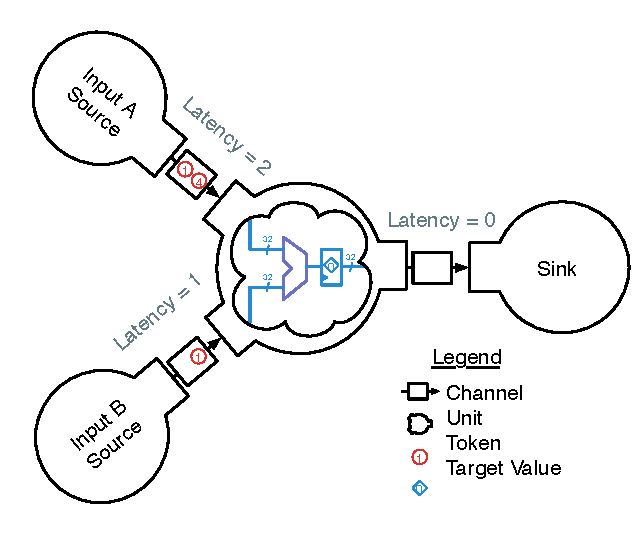
\includegraphics[width=\columnwidth]{figures/adder-example1.pdf}
%        % graffle3pdf -c initial-state midas-graphics/graffle/adder-example.graffle figures/adder-example1.pdf
%    \end{subfigure}
%    \begin{subfigure}[t]{0.32\textwidth}
%        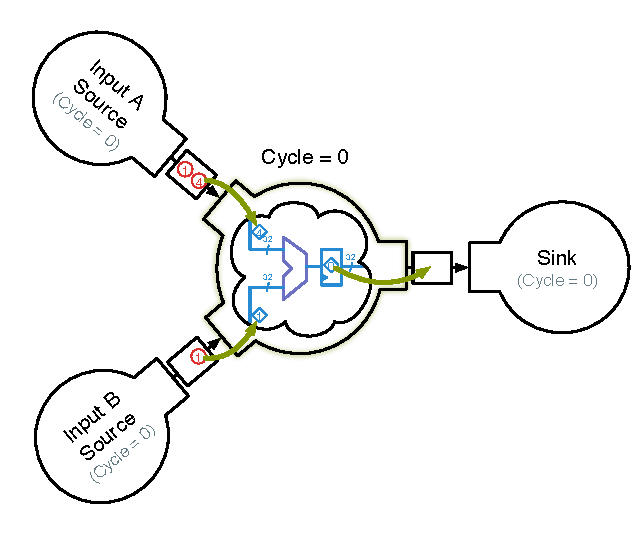
\includegraphics[width=\columnwidth]{figures/adder-example2.pdf}
%        % graffle3pdf -c tfire-cycle0 midas-graphics/graffle/adder-example.graffle figures/adder-example2.pdf
%    \end{subfigure}
%    \begin{subfigure}[t]{0.32\textwidth}
%        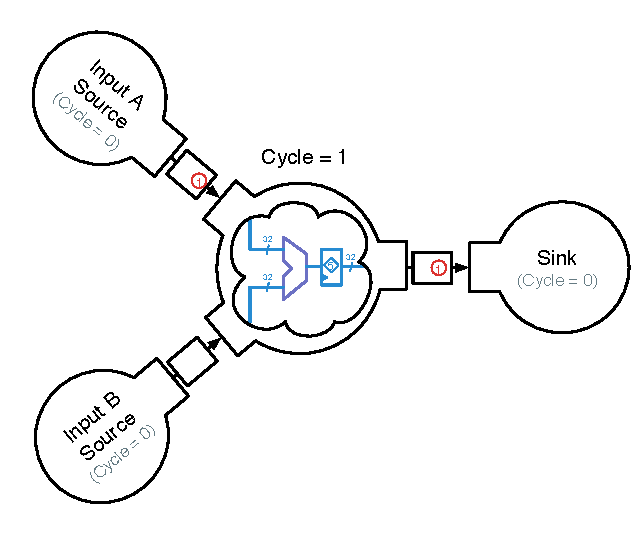
\includegraphics[width=\columnwidth]{figures/adder-example3.pdf}
%        % graffle3pdf -c cycle-1 midas-graphics/graffle/adder-example.graffle figures/adder-example3.pdf
%    \end{subfigure}
%	\centering
%    \caption{A 32-bit adder and environment simulating a single cycle of target time.}
%    \label{fig:adder-example}
%\vspace{-0.1in}
%\end{figure*}
%
%Figure~\ref{fig:adder-example} illustrates an example graph, consisting of a
%single 32-bit adder unit, composed with source and sink units, as it executes
%one cycle of target time.

A simulator that faithfully implements this graph decouples target time from
host time. Unlike in an FPGA prototype, where every FPGA clock cycle emulates a
target clock cycle, an FPGA-hosted model only executes a target-clock-cycle when
it can legally fire. Thus, the behavior of the target is decoupled from the
host, allowing simulators to be partitioned across the host and to tolerate
variable-host-latencies to DRAM and the CPU, while remaining deterministic.
Unfortunately, this results in target time advancing slower than it would in an
FPGA prototype of the same host frequency.  This is quantified by the
FPGA-cycle-to-Model-cycle Ratio~(FMR)\cite{APortNetworks}, below, which increases from
one~(the simulator simulates a target cycle on every FPGA host cycle) as the simulator stalls on token availability and backpressure. The FMR
of a simulator is variable: it is a function of both application-dependent
behavior in the target and variable latencies in host services.
$$ FMR = \frac{Cycles_{FPGA}}{Cycles_{Target}}$$

\section{The \SIMNAME Compilation Flow}\label{sec:fame1}
\SIMNAME-generated simulators compose three types of models in their target graphs:
\begin{enumerate}
    \item \emph{Transformed RTL} models generated from ASIC RTL.
    \item \emph{Abstract RTL} models intended for FPGA hosts.
    \item \emph{Software} models that are hosted on a CPU.
\end{enumerate}

The next three sections give an overview of how \SIMNAME, with the help of the
user, maps a target graph composed of these models into an FPGA-accelerated
simulator.

\subsection{ASIC-RTL-to-Model Transformation}\label{sec:fame1}
We transform a synchronous block of RTL into a model using a FIRRTL~\cite{firrtl} transformation called a \emph{FAME-1}
transform. The transformation gates state update of the RTL with a model-global
signal, \emph{targetFire}, which is driven with the AND-reduction of the valid
signals of all input ports and the ready signals of all output ports.  Thus, in
these models, state update, output token enqueue, and input token dequeue occur
simultaneously in a single host-clock-cycle.

\subsection{FPGA-Host Mapping}

Once ASIC-RTL has been transformed into models, \SIMNAME creates a host-agnostic
mapping of the target graph. This is also the point where \SIMNAME links in
other models, including \PNAME instances.

Using Chisel, \SIMNAME generates simulation FIFOs that implement the channels of
the target graph.  When a channel spans the boundary of the FPGA, \SIMNAME
generates an \emph{endpoint}, a FIFO with a matching head or tail on the
opposite part of the host platform.  Together, these endpoints implement the
simulation channel.  All remaining I/O on transformed-RTL models
are bound to a default I/O model, which acts as an infinite source and sink of
tokens.  During this process, \SIMNAME also generates memory-mapped modules for
simulation control and instrumentation. These include a DRAM-initialization
module and a master that governs the advance of target time on the FPGA.

\begin{figure}[t]
    \centering
    \includegraphics[width=\columnwidth]{figures/target-graph.pdf}
    % graffle3pdf -c target-graph midas-graphics/graffle/masters-target.graffle figures/target-graph.pdf
    \caption{The graph of target designs studied in this paper.}
    \label{fig:default-target}
\end{figure}

Once all of the simulation components have been generated, the simulation
interconnect is elaborated and bound to a single AXI4 slave port. All
memory-mapped simulation components are accessed through this
interface. Additionally, a crossbar is generated to arbitrate between components
that require FPGA-host DRAM. Ultimately, \SIMNAME emits a Verilog file and a
C++ header describing the simulator's memory map. To generate a bitstream, the
user instantiates the \SIMNAME-generated Verilog in a skeleton FPGA project
that exposes AXI4 interfaces to the FPGA's off-chip memory systems and
interconnect to the host CPU.

\subsection{Software Simulation Driver \& Software Models}
To control the simulator, the user writes a C++ program that links against the
\SIMNAME C++ libraries and the generated header. The \SIMNAME libraries implement
basic commands used to control simulation.  These commands are decomposed into
memory-mapped I/O issued over the simulation interconnect.  To complete
the simulator, the user links in software models into this program.

\section{Targets \& Hosts of This Paper}\label{sec:targetandhostmachines}

All target designs used in this work are tethered RISC-V processors with a
single-channel DRAM subsystem.  They share the target graph shown in
Figure~\ref{fig:default-target}. This graph comprises a Rocket-Chip-generated
transformed-RTL model that includes one to four Rocket pipelines with L1 caches
and a cache-coherence controller; software models for a UART~(not shown),
a block device, and the RISC-V front-end server
(FESVR, which provides BIOS-like functionality); and a \PNAME instance,
which connects to an AXI4 port presented by the processor.  All remaining I/O
of the transformed-RTL model, including reset, is bound to the default I/O
model.

\begin{figure}[t]
    \centering
    \includegraphics[width=\columnwidth]{figures/mapped-simulator.pdf}
    % graffle3pdf -c f1 midas-graphics/graffle/masters-target.graffle figures/mapped-simulator.pdf
    \caption{The target mapped to an F1 host. The contribution of this work is
    the \PNAME instance, which replaces a crude latency-pipe model provided
    by the prior work.}
    \label{fig:mapped-simulator}
\end{figure}

While \SIMNAME supports other FPGA hosts, currently FireSim only has support for
Amazon EC2 F1 instances. F1's \texttt{f1.2xlarge} instances have a Xilinx
UltraScale+ XCVU9P\footnote{2.6 million logic cells, \wunits{346}{Mb} of
on-chip memory.}
attached to four \wunits{16}{GiB} channels of ECC-enabled DDR4 SDRAM.  FPGAs
are attached to a CPU with 8 hardware threads and \wunits{112}{GiB} of
DRAM. Figure~\ref{fig:mapped-simulator} shows the target mapped to an F1 host.

%
%\chapter{Memory Model Architecture}
%
%%% This section describes the design of the memory system model. How host target
% decoupling is achieved. What configurations are available.
\PNAME is a \textit{generator}, written in Chisel~\cite{Chisel}, that can
elaborate \textit{instances} from a space of possible parameterizations.
Instances themselves model a space of different memory systems: the user picks the
final target-design point by programming the instance's configuration registers
at runtime.

As input, \PNAME accepts a parameterization that constrains features
of the instance, such as its interface widths, the maximum number of
outstanding requests it must support, and the type of memory system the
instance will model (a \emph{timing-model class}). As output, \PNAME generates
an instance RTL module and memory map of its host configuration registers. These
registers control timing parameters; their values can be modified at runtime
to reconfigure the instance without needing to recompile the FPGA bitstream.

\section{Instance Organization}

\begin{figure}[t]
	\centering
	\includegraphics[width=0.8\textwidth]{figures/memory-model-block-diagram.pdf}
     % graffle3pdf -c full midas-graphics/graffle/memory-model-block-diagram.graffle figures/memory-model-block-diagram.pdf
    \caption{A block diagram of a \PNAME instance, with all signals
    that may stall timing model execution illustrated.}
	\label{fig:timing-model}
\end{figure}

The block diagram of an instance is shown in Figure~\ref{fig:timing-model}.
Instances operate by using the FPGA host's DRAM as a backing store.  Target
requests carried in simulation tokens are snooped by the \emph{host-request
scheduler}, which issues them to the host memory system.  Responses from the
host memory system are subsequently buffered in the \emph{host-response
staging} modules. In parallel, the \emph{timing model}, a simulation model
transformed from target-time RTL using a FAME-1 transform, consumes input
tokens and generates output tokens. When the timing model wishes to release a
valid memory-response token, it queries the host-response staging module for
the corresponding host response. If the host memory system has not yet responded,
\texttt{targetFire} is de-asserted, preventing token flow and
ultimately stalling the simulator. We describe this mechanism in greater detail in
the next section~(\ref{sec:memory-model-operation}).

The host-request scheduler and host-response staging modules, together with the
FPGA-host DRAM, constitute the functional model of an instance.  Timing models
are written in target-time RTL and have three interfaces:

\begin{enumerate}
    \item An AXI4 port through which the model receives memory requests from the rest of the target.
    \item Two functional-model request ports~(BREQ \& RREQ) through which the
        timing model fetches data for target responses from the host-response
        staging module. Responses are carried by the next tokens~(fTokens)
        generated by the host-response staging unit.
    \item A host-configuration port that carries the timing parameters of the
        model and records instrumentation data.
\end{enumerate}

During instance generation, \PNAME binds the host-configuration port to memory-mapped
registers on the simulation bus. It then FAME-1-transforms the timing model, connects it to
token queues, and binds the \texttt{targetFire} signal, which is asserted when all of the following
conditions hold:

\begin{enumerate}
    \item All input tokens are present~(\textit{iTokens valid} in Figure~\ref{fig:timing-model}).
    \item All output queues are ready~(\textit{outputs ready}).
    \item The host-request scheduler can accept a request~(\textit{HRQ ready}).
    \item All host-response tokens are present~(\textit{fTokens valid}).
\end{enumerate}

\section{Operation}\label{sec:memory-model-operation}

\begin{figure*}[t]
	\centering
    \begin{subfigure}[t]{0.23\textwidth}
        \includegraphics[width=\columnwidth]{figures/model-operation-1.pdf}
        % graffle3pdf -c 1 midas-graphics/graffle/memory-model-operation.graffle figures/model-operation-1.pdf
        \caption{}
        \label{fig:model-operation-1}
    \end{subfigure}
    \begin{subfigure}[t]{0.24\textwidth}
        \includegraphics[width=\columnwidth]{figures/model-operation-2.pdf}
        % graffle3pdf -c 2 midas-graphics/graffle/memory-model-operation.graffle figures/model-operation-2.pdf
        \caption{}
        \label{fig:model-operation-2}
    \end{subfigure}
    \begin{subfigure}[t]{0.24\textwidth}
        \includegraphics[width=\columnwidth]{figures/model-operation-3.pdf}
        % graffle3pdf -c 3 midas-graphics/graffle/memory-model-operation.graffle figures/model-operation-3.pdf
        \caption{}
        \label{fig:model-operation-3}
    \end{subfigure}
    \begin{subfigure}[t]{0.23\textwidth}
        \includegraphics[width=\columnwidth]{figures/model-operation-4.pdf}
        % graffle3pdf -c 4 midas-graphics/graffle/memory-model-operation.graffle figures/model-operation-4.pdf
        \caption{}
        \label{fig:model-operation-4}
    \end{subfigure}
	\centering
    \caption{A \PNAME instance simulating a single-target-cycle read. Data
    tokens carry target transactions~(their target-valid bit is set) whereas
    empty tokens do not carry a target transaction.}
    \label{fig:model-operation}
\end{figure*}

To demonstrate how \PNAME instances operate, let us consider an instance with a
single-cycle-memory timing-model. This is depicted in Figures~\ref{fig:model-operation-1}-\ref{fig:model-operation-4}.

Suppose we have reached the first read request issued to the memory
system~(Figure~\ref{fig:model-operation-1}).  Let this be host and target cycle
0. When the timing model accepts this request, it is snooped by
host-request scheduler.  Simultaneously, the timing model makes a request
to host-response staging module as it needs to reply to the read in the next
target cycle.

In host cycle 2~(Figure~\ref{fig:model-operation-2}), the host-response staging module cannot produce
the associated host response, since it has yet to be issued, and so generates
no fToken, stalling the timing model. In parallel, the host-request scheduler
issues the required read to the host memory system.
While the host-response staging module waits, the timing model
stalls. If the host memory system responds in $K$ cycles, at host
cycle $K+1$~(Figure~\ref{fig:model-operation-3}), that response is received.

In cycle $K+2$~(Figure~\ref{fig:model-operation-4}), the host-response staging module produces an
output token, targetFire is asserted, and target cycle 1 executes. Here the
timing model forwards the data directly into its output token.
From the target's perspective, the read occurred in a single cycle, however,
the cycle was executed with an FMR of $K+2$.  As the latency of the
target increases, FMR decreases and approaches unity.  If the
target memory system is strictly slower the host memory system, the instance
executes at unity FMR.

\section{Functional Model Configuration}\label{egress}
Our design allows both the host memory system and the timing model to reorder
responses; the host-staging unit implements a set of virtual queues for each
AXI4 channel. Each queue represents the FIFO ordering within a single channel
ID. The size of the functional model is sensitive to the maximum number of reads
and writes it must accept, the maximum number of transactions that can be in
flight on the same ID, and the maximum request lengths. For small degrees of ID
reuse, or small numbers of outstanding requests, the memory system model
implements each virtual queue as a physical queue, and aggregates them together in one dual-ported
BRAM~\cite{LIFPGADesign}. For greater numbers of AXI IDs or greater degrees of ID
reuse, it dynamically assigns entries within block RAMs, and maintains a
hardware linked list to track to read-response order in a given ID.

\section{Providing Deterministic Functional-Model Behavior}
By default, instances forward target requests directly to the host-memory
system, under the assumption there will never be reads and writes to the same
address in flight\footnote{In AXI4, the value a read returns when a write to
the same address is in-flight is implementation defined.}. When a buggy target
exhibits this behavior, the host memory-system is free to reorder these
requests, introducing non-determinism. To help debug targets that behave this
way, the host-request scheduler provides a strict mode in which it orders reads
and writes---issuing writes only when no reads are in flight, and reads only
when there are no writes in flight.

\section{General-Purpose Timing-Model Classes}\label{sec:timing_model}

\PNAME provides two simple, general-purpose timing-model-classes that can be used to
model large off-chip memory systems. The first is a \emph{latency-bandwidth
pipe}~(LBP) that applies independently programmable latencies to read and write
requests and will not accept any new requests beyond a programmable limit. The
second is a \emph{bank-conflict} model, which adds a penalty of $max(0, t_{CP} -
t_{\Delta})$ cycles to a base latency if the bank was used
$t_{\Delta}$ cycles prior, where $t_{CP}$ is the maximum conflict penalty.
These models were validated in trace-driven RTL simulation against
software golden models which match their cycle-by-cycle behavior exactly.  We
give the FPGA resource utilization for a handful of
instances in Table~\ref{tbl:lbp-model-resources}\footnote{We
used Vivado 2017.1, targeting the XCVU9P-FLGB2104-2-i device present on F1
instances. We registered all I/O, and overconstrained the design
to \wunits{400}{MHz} to obtain a best-case $f_{MAX}$. We exclude memory
LUTs~(lightly used) and DSP48s~(unused).}.

\begin{table}[htb]
\centering
    \begin{tabular}{c c c c c }
	\hline
        \textbf{Example Instance} & Logic LUTs & FFs & BRAM & $f_{MAX}$ \\
	\hline
        8 read, 8 write & 1337 & 972 & 3 &  281 \\
        32 read, 32 write & 2119 & 1500 & 1 & 264 \\
        Above w/ no ID reuse & 1289 & 873 & 1 & 317 \\
	\hline
	\end{tabular}
    \caption{Resource counts and best-case $f_{MAX}$~(MHz) for three different
    LBP models (maximum AXI4 burst length of 8 beats). Supporting more concurrent transactions~(row 2) requires a larger
    functional model; this can be mitigated by giving the generator hints~(row 3).}
\label{tbl:lbp-model-resources}
\end{table}

\section{Composable Last-Level-Cache Model}
All timing model classes can be generated with a single-banked, write-back,
last level cache~(LLC) model with a random replacement policy.  Since we can
reuse the same functional model, the model only instantiates tag and metadata
arrays, letting us model an LLC that would be too
large to fit on the FPGA. \PNAME LLC models have a runtime-configurable number of sets
and MSHRs, associativity, and line size. Refills from the backing memory model
are prioritized over reads over writes. Reads or writes made to a set with a
pending writeback or refill are interlocked.  We make the cache composable with
all other timing-models by implementing an additional internal AXI4
bus~(stripped of its data fields). We give the FPGA resource utilization for a
handful of LBP-backed LLC instances in
Table~\ref{tbl:llc-model-resources}.
\begin{table}[htb]
\centering
    \begin{tabular}{c c c c c}
	\hline
        \textbf{Example Instance} & Logic LUTs & FFs & BRAM & $f_{MAX}$ \\
	\hline
        4 MiB, 16 ways & 2166 & 1240 & 27 & 222 \\
        4 MiB, 8 ways  & 2265 & 1272 & 39 & 220 \\
        4 MiB, direct mapped & 1848 & 1241 & 34 & 242 \\
        64 MiB, 8 ways & 2545 & 1426 & 251 & 152 \\
	\hline
	\end{tabular}
    \caption{Resource counts and best-case $f_{MAX}$~(MHz) for four different
    LBP-backed LLC models, labeled with the largest capacity and associativity they can model~(128B cache lines).}
\label{tbl:llc-model-resources}
\end{table}

We validated the LLC model in RTL simulation backed with a latency bandwidth
pipe. We generated trace-based microbenchmarks and measured cache behavior
for a set of generated instances programmed with runtime settings.

%
%\chapter{On DRAM Memory Systems}
%
%%Before describing \PNAME's DRAM timing-models~(Chapter~\ref{sec:dram-timing-model}), we review some relevant background
on DRAM memory systems.

\section{DRAM Device Architecture}\label{sec:dram-arch}
In a DRAM IC, arrays of bit cells are hierarchically arranged into multiple
parallel \textit{banks}. Banks provide the primitive level of concurrency in a
DRAM memory system: they can service independent requests assuming they do not
simultaneously require shared resources like the data, address and command
buses.  Multiple DRAM ICs can be arranged in parallel to widen the data bus;
address and command buses fan out to each IC.

A basic DRAM operation requires a series of three commands: \textit{activate (ACT)},
\textit{column access (CAS)}, and \textit{precharge (PRE)}. The ACT command
enables the word-lines of the array corresponding to a single \textit{row} of
the bank. The cells of the row are sensed and saved in a \textit{row
buffer}. A CAS command then selects a subset of the row buffer to
read or write; data is bursted over successive clock edges. While the row
buffer remains \textit{open}, the row can be accessed by issuing new CAS
commands. To access a different row, a PRE command must be
issued to \textit{close} the row and recharge the bit-lines.
The organization of a typical DRAM device is shown in Figure~\ref{fig:dram-device}.

\begin{figure}
	\centering
	\includegraphics[width=0.8\textwidth]{figures/dram-device.pdf}
     % graffle3pdf -c device midas-graphics/graffle/dram-diagrams.graffle figures/dram-device.pdf
    \caption{The organization of a typical DRAM device.}
	\label{fig:dram-device}
\end{figure}

DRAM gradually loses its stored state over time as bit cell capacitors leak. To
maintain their state, DRAM cells must be periodically refreshed. In the DDR
standards, JEDEC mandates that cells must be refreshed once every 64
ms. Since activations to every row cannot generally be guaranteed during normal
use, DRAM devices are refreshed explicitly with a refresh command~(REF). To
reduce complexity, this command refreshes a constant number of contiguous rows
in all banks concurrently. DRAM manufacturers generally have kept the number of
refresh commands required to iterate through the entire array constant: 8192
commands per 64 ms interval, or one every 7.8 $\mu s$.
% is there a citation for this ^
\section{DRAM Controller Architecture}\label{sec:dram-mas}
A DRAM controller is responsible for responding to memory
requests from one or more requesters by scheduling those requests over its
memories as a judicious stream of DRAM commands.

Memory access scheduling~(MAS) is the process by which, for a given cycle, a
controller selects a single DRAM command to be issued from a legal set. Legal
commands are constrained by the current state of each bank, the availability of
shared resources like the command and data buses, and timing constraints
imposed by the DRAM devices. Good MAS policies strike a balance
between minimizing latency, maximizing bandwidth, minimizing power, and
maintaining quality-of-service guarantees. In this paper we consider two common
MAS policies: First-Come First-Served~(FCFS) and First-Ready
FCFS~(FR-FCFS)~\cite{frfcfs}.

In a FCFS MAS, commands for the oldest pending memory reference are issued
first. This is the simplest MAS policy, but tends to under-utilize available
DRAM bandwidth as younger requests that may hit an open row buffer must wait
behind commands that miss. In a FR-FCFS MAS, first, ready~(legally issuable) column
commands are prioritized over ready row commands. Second, commands for older
references are prioritized over younger ones. This permits younger but ready
column commands to be issued before older row commands, improving DRAM bandwidth
utilization considerably.

%\section{Power Consumption in DRAM Memories}\label{sec:dram-power}
%
%DRAM power consumption can be divided into six different classes: activation
%(including precharge), read, write, termination, refresh, and background power.
%
%Activation is generally the largest component of DRAM power consumption.  In an
%effort to maximize areal density and reduce cost-per-bit, DRAM sub-arrays have
%long, high capacitance bitlines, which are driven to VDD or ground during the
%restore phase of an activation. Moreover, DRAM rows are long: thousands of
%bitlines are simultaenously charged or discharged in a single activation. These
%two properties lead to high peak-current draw during an activation. In order to
%stay within a power envelope where DRAM devices can be cooled passively without
%heatsinks, DRAM manufacturers put limits on activation frequency through
%$t_{RRD}$ and $t_{FAW}$ constraints (see table\ref{tbl:dram-timings}).
%
%Read and write power consumption accounts for the power dissipated as data is
%driven between the I/Os of the chip and its various sub-arrays, as well as the
%power used to decode the read or write command.
%
%Refresh power accounts for the power lost during the successive activations and
%precharges of a refresh command. It is a growing component of power consumption
%as modern DRAM devices trend towards higher row counts. Higher row counts impose
%that more rows must be refreshed per command which forces the device to spend
%more time in refresh (higher $t_{RFC}$).
%
%Termination power accounts for the power dissipated in on-die termination
%resistors of a device during a write, and by the output buffers of a device
%during a read. In multi-rank systems, this also includes power dissipated in
%the termination resistors of ranks not being addressed.
%
%Finally, background power accounts for leakage of various circuits within the
%IC. Here there are two dimensions of note. First, activated banks
%leak more than precharged banks. Second, powered-down ranks~(CKE low) leak less
%than powered-up ranks~(CKE high).


\section{DRAM Memory System Simulators}

The current state of the art in DRAM simulation in academia is cycle-accurate
software simulators like~\cite{dramsim, ramulator, usimm}. These simulators
generate DRAM command streams that have been validated against industrial
models. In trace-driven mode, operating at full throughput and only as a
timing-model, these models simulate at rates of
hundreds of KHz to ones of MHz~(reported in \cite{ramulator}).
%
%To model power dissipation, Micron white papers~\cite{micronpower} describe a strategy that
%assigns an average current draw to different modes of power dissipation. Micron
%has encoded this in freely available spreadsheets that generate estimates based
%on system-level measurements of DRAM activity, such as row-buffer hit rate.
%DRAMSim2 directly implements the Micron approach by integrating the appropriate
%current based on the state of the memory system.

%One limitation of the Micron approach, is that it does not account for the
%power dissipation of the controller itself. However, for modest memory
%controller implementations, this should be small.

% OLD DRAM Section
%We will now review important first-order architectural
%characteristics of DRAM memory-systems that we model in our initial set of
%timing models.
%
%\subsection{DRAM Device Architecture and Organization}
%
%In a DRAM IC, arrays of bit cells are hierarchically arranged into multiple
%parallel \textit{banks}. Banks provide the primitive level of concurrency in a
%DRAM memory system. They can service independent requests, assuming they do not
%simultaneously require shared resources like the data, address and command
%buses.  Multiple DRAM ICs can be arranged in parallel to widen the data bus;
%address and command buses fan out to each IC.
%
%A basic DRAM operation requires a series of three commands: \textit{activate (ACT)},
%\textit{column access (CAS)}, and \textit{precharge (PRE)}. The ACT command enables the word-lines of the array corresponding to a single \textit{row} of the bank. The cells of the row are
%sensed and saved in a \textit{row buffer}(typically O(1) kB). A CAS command then selects a subset
%of the row buffer to read or write; data is bursted over successive clock edges. While the row
%buffer remains \textit{open}, the row can be accessed by issuing new CAS commands. To access a
%row not stored in the buffer, a PRE command must be issued to \textit{close} the row and charge
%the bit-lines for a new access.
%
%\subsection{DRAM Controller Architecture}
%
%At the highest level, a DRAM controller is responsible for responding to memory
%requests from one or more requestors by scheduling those requests over its
%attached memories as a judicious stream of DRAM commands.
%
%Memory access scheduling (MAS) is the process by which, for a given cycle, a
%controller selects a single DRAM command to be issued from a legal set. Legal
%commands are constrained by the current state of each bank, the availability
%of shared resources like the command and data buses, and timing constraints
%imposed by the DRAM standard. Good MAS policies strike a delicate balance
%between minimizing latency, maintaining quality-of-service guarantees across
%multiple threads of execution, maximizing bandwidth, and minimizing power.
%There are plethora of academic papers on MAS policies, and still more
%industrial patents on the subject. We outline some of the most popular MAS policies
%here.
%
%\subsection{First-Come First-Serve (FCFS) Policy}\label{fcfs}
%Commands for the oldest pending memory reference are always issued first. This
%is the simplest MAS policy, but one that grossly under-utilizes available DRAM
%bandwidth. FCFS schedulers are common in older machines, and those that present
%few concurrent memory requests.
%
%\subsection{First-Ready FCFS (FR-FCFS)\cite{frfcfs} Policy}\label{frfcfs}
%First, column access commands that hit in an open row-buffer are prioritized,
%then row and precharge commands from the oldest pending reference are
%considered.  FR-FCFS is a relatively simple scheme that achieves far higher BW
%than FCFS. It is the de facto standard against which new MAS policies for
%machines with a single stream of memory references (like single-core
%out-of-order machines), are compared.
%
%\subsection{DRAM Software Simulation}
%
%The current state of the art in DRAM simulation in academia are cycle-accurate
%software simulators like DRAMSim2\cite{dramsim}, Ramulator\cite{ramulator} and
%USIMM\cite{usimm}. These models generate DRAM command streams that
%have been validated against industrial models (for some standards). Both
%Ramulator and DRAMSim2 can be easily integrated into Gem5\cite{gem5}, though it
%includes a detailed event-based model of its own\cite{gem5event}. In trace-driven mode, operating at full throughput and only as a timing model, these
%cycle-accurate models simulate at frequencies ranging from 100s of KHz to ones
%of MHz\cite{ramulator}.

%\subsection{DRAM Power Modeling}

%In order to model power, Ramulator relies on DRAMPower\cite{drampower}, to which it passes its command trace. Micron describes strategies in their technical notes for estimating DRAM power\cite{micronpower} (which DRAMSim2 employs). They also made these calculations accessible by providing spreadsheets that take micro-architectural event frequencies as input. These approaches can carry over to FPGA simulation, as sufficiently detailed FPGA models can add instrumentation for these events, while simpler models can save the memory access trace to a buffer and compute power out-of-band\cite{strober}.

%
%\chapter{DRAM Timing Models}\label{sec:dram-timing-model}
%
%%\input{tex/dram-timing-model}
%
%\chapter{Experimental Setup}
%
%\input{tex/methodology}
%
%%\chapter{Demonstrating \textsc{FASED}}\label{sec:evaluation}
%
%\input{tex/evaluation}
%
%\chapter{Conclusion}
%
%%Our goal in building out the FireSim project was to build a radically
inexpensive, yet fast and productive, cycle-accurate full-system simulation
technology to attack a key contributor to the NRE of building silicon.  While
our system is most similar to existing hardware emulators, our approach is
unique in that is uses a single COTS FPGA, and depends on a completely open
source toolchain. However, it was difficult to make this comparison in good
faith, as early versions of FireSim had two critical limitations: were limited
to supporting to small, single-clock domain.

We designed Golden Gate to address these limitations~(Chapter~\ref{sec:golden-gate}). First, Golden Gate uses a LI-BDN
target formalism and RAMP-inspired multi-cycle optimizations to fit larger SoCs
on a single FPGA; descriptions of these optimizations can be found in Albert
Magyar's dissertation. Overcoming the clocking limitations was the primary focus of this dissertation.
To model multiple clock domains, we introduced a new FAME transform that avoid
using dedicated FPGA clock resources like prior academic work, in favor of a
clock-gating scheme that should be portable to many different FPGA
platforms~(Chapter~\ref{sec:static-multiclock}.  To model clock switching an
generation circuits, which form the basis of dynamic frequency scaling support
in realistic SoCs, we introduced a timestamped subgraph into the simulator that
implements a conservative PDES~(Chapter~\ref{sec:dynamic-multiclock}).

One takeaway from our work in supporting clock switching and generation
structures is that closely coupled clock-generating circuits, like ICGs and
clock multiplexors, are probably best simulated \emph{in situ}, instead of
being extracted into a decoupled unit. State for these circuits can be left in
the target, and combinational functions they perform on clocks can be hoisted
into the hub-unit's second stage to act on future clock enables. This would
generate new clock buffers for these derived clocks. This clearly would be
insufficient for modelling clock generators like PLLs that can't be described
as digital functions on existing clocks, like PLLs.  For modelling this class
of circuits, having an independent TU unit seems entirely sensible.  This
hybrid approach would also reduce the number of timestamped inputs on the hub
unit, addressing a potential scalability challenge in systems with many clocks.
Implementing and studying this approach is the logical continutation of the
work described in this dissertation.

While Golden Gate has made inroads in simulating far more realistic SoCs in
FireSim, there are still many domains under the FireSim project that require
attention.  First, FireSim should be ported to other FPGAs to verify our claims
about the flexibility of our approaches. Here there are ongoing efforts, both
at Berkeley and abroad. Perhaps the biggest frontier for innovation lies in
improving FireSim's debuggability. Snapshotting features, to provide greater
visibility over the target, are important tool in commerical hardware
emulators. Earlier verions of MIDAS had support for this, but that
implementation presupposed a monolithic, single-clock domain hub and used a
scan chain that increased FPGA resource utilization.  Supporting
resource-efficient state capture that co-exists with resource optimizations is
both an important and compelling avenue for future work.

FireSim's growing userbase of both industrial and academic users, suggests our
vision for a more cost-effective full-system simulation technology addresses a
material technology gap. We hope that FireSim and the contributions of this
dissertation inspire more academic research in to better open-source hardware
emulation systems in the future.


\printbibliography

\end{document}
